\documentclass{article}

%----------------------------------------------------------------------------------------
%	PACKAGES AND OTHER DOCUMENT CONFIGURATIONS
%----------------------------------------------------------------------------------------

\usepackage[T1]{fontenc}
\usepackage[utf8]{inputenc}
\usepackage{lmodern}
\usepackage[english]{babel}
\usepackage[autostyle]{csquotes}
\usepackage{graphicx} % Required for inserting images
\usepackage[hyphens]{url}
\usepackage{hyperref}
\usepackage{amsmath}      % for additional mathematical features
\usepackage{amsfonts}     % for mathbb command
\usepackage{float}
\usepackage{setspace}
\usepackage{listings}
\usepackage{rotating}
\doublespacing
\usepackage[backend=biber,style=authoryear]{biblatex}
\renewcommand*{\bibfont}{\small}
\addbibresource{Bibliography.bib}
\usepackage{tcolorbox}
\usepackage{amssymb}

%----------------------------------------------------------------------------------------
%	DOCUMENT MARGINS
%----------------------------------------------------------------------------------------

\usepackage{geometry} % Required for adjusting page dimensions and margins

\geometry{
	paper=a4paper, % Paper size, change to letterpaper for US letter size
	top=3cm, % Top margin
	bottom=3cm, % Bottom margin
	left=3cm, % Left margin
	right=3cm, % Right margin
	headheight = 10pt, % Header height
	footskip = 1.5cm, % Space from the bottom margin to the baseline of the footer
	headsep = 1.2cm, % Space from the top margin to the baseline of the header
	%showframe, % Uncomment to show how the type block is set on the page
}

%----------------------------------------------------------------------------------------
%	SECTION TITLE APPEARANCE
%----------------------------------------------------------------------------------------


\title{Diversity as a management tool for forest ecosystem services \\ 
\large A theoretical exploration using control theory and viability analyses}
\author{Clementine de Montgolfier}
\date{Dec 2023}

\begin{document}

\maketitle

\section{Summary}

Defining optimal forest management strategies in a changing world is a challenge in the field of forest ecology. The complexity of forest ecosystems, coupled with the uncertainty of future climate conditions, makes it difficult to determine the best course of action. The concept of forest diversity is a key consideration in this debate, as it is believed to be a significant factor in the resilience of forest ecosystems. This study aims to explore whether diversity can be used as a management tool to maintain the ecosystem in a desirable state. To this end, we will use a theoretical model of a mixed-species, multi-layered forest, and apply control theory and viability analyses to assess the relationship between diversity and management trajectories, considering both species and vertical diversity at the stand level. RESULTS\\

\noindent \textbf{Keywords:} forest management, diversity, control theory, viability theory

\section{Intro}

\subsection{Forest and management, new practices for new challenges}

Forest covers 31\% of the territory in France, however forest health metrics show rapid degradation  marked by an alarming +80\% increased mortality rate, a 4\% decline in growth and a deceleration in carbon storage due to the growing number of health crises combined with more frequent droughts ~\autocite{IGN}. This impacts forest composition, structure, dynamics and the provisioning of ecosystem services to human populations (Climate regulation, water purification, wood production, air quality, cultural leisure...) ~\autocite{grammatikopoulouValueForestEcosystem2021}. Notably, 94\% of these forests are designated as productive, emphasizing the critical need to adapt management strategies to address these emerging challenges. 
New adaptative policy actions are studied to robustly sustain the state of these forests as the adaptation from monospecific forets stand with clear-cutting into mixed species and uneven aged forest stand with a diversity of selectives logging practices  ~\autocite{REFSautre, raymondIrregularShelterwoodSystem2009}. Knowledge of these nexw practices is still limited but they are already implemented relying on the idea that diversification is a way to increase multiple ecosystem services ~\autocite{tilmanBiodiversityPopulationEcosystem1996}.

For obvious economic constraints sustainable wood extraction has been the primary driver of forest management practices. With this approach diversity indices are treated as auxiliary metrics, preventing interference with the core objective of wood extraction. The pivotal question that emerges is whether we can redefine this paradigm and choose diversity as our primary constraints to explore potential benefits and differences in our management approaches.This paradigm shift is motivated, firstly, by the insights from Biodiversity-Ecosystem Functioning (BEF) studies, which highlight diversity as a critical component for overall ecosystem health. The second drive of our study is the proposition that forest management itself can transform into a purposeful tool to enhance diversity within these ecosystems. Our study's second motivation is the indicating that forest management can function as a tool to actively enhance diversity within ecosystems.

But given the many uncertainties in climate and complex response of forest systems to management actions, models and decision science should be called upon to assist their design.

Particularly to understand the link between climate change, biodiversity, levels of a diversity of ecosystem services and management practices. \\

\subsection{Diverstity and ecosystem functionning}

Work on composition diversification and its effects is mainly driven by the first work on biodiversity ecosystem functioning (BEF) from grassland studies ~\autocite{tilmanBiodiversityPopulationEcosystem1996}.They showed that there was a positive link between biodiversity and ecosystem functioning. But the mechanisms behind this link are still not well understood. Numerous hypothesis were made to explain this link: competitive exclusion, niche complementary, sampling effect, etc. ~\autocite{aliBiodiversityEcosystemFunctioning2023}. This uncertainty makes it difficult to predict the impact of biodiversity loss.
While the hypothesis of BEF relationship, and its relevance is still debated, it fuels an entire segment of research.
The study of BEF in forest is more recent and mainly focused on the link between species diversity and productivity. A positive relationship has been demonstrated at a global scale ~\autocite{liangPositiveBiodiversityproductivityRelationship2016}, but also in specific forest ~\autocite{morinTreeSpeciesRichness2011,paquetteEffectBiodiversityTree2011,jourdanManagingMixedStands2021}. But the interaction is not positive in every forest type. ~\autocite{forresterReviewProcessesDiversity2016}.
However one of the way to explain the contrasting results could be that the biodiversity-productivity interaction is context dependant. The relationship seems to be mostly positive in harsh climate and low tree density but negative in suitable environment ~\autocite{juckerClimateModulatesEffects2016}.

It is also reductive to consider productivity as the only characteristic of forest ecosystems, and many other should be accounted for : support of habitat and biodiversity, regulation of flood, carbon storage and also cultural and aesthetic values.
All of them might not be impacted in the same way. For example there doesn't seem to be an effect of mixture on other soil biodiversity ~\autocite{korboulewskyHowTreeDiversity2016}.
To have a better understanding of the impact of biodiversity on forest functioning it seems necessary to study multiple functions at the same time. It has been shown that diversity can increase multi-functionality by the jack-of-all-trades and master of none mechanism ~\autocite{vanderplasJackofalltradesEffectsDrive2016} while not optimizing any of them. With this blindly increasing biodiversity can increase forest multi-functionnality without optimizing any of them and leading sometimes to trade-offs. This multifunctionnality is not only linked to species identity but can also come from different life stage of the same species. For instance, tade-offs can be observed in the balance between young and old grown forests, if the former are more productive, they store less carbon than the latter ~\autocite{caspersenSuccessionalDiversityForest2001}. It is thus important to define the functions that we want to preserve as well as threshold for each of them. Thus vertical diversity brought back in forest by uneven forest management have also been advocated to be a possible solution to the increasing vulnerability of this ecosystem ~\autocite{guldinRoleUnevenAgedSilviculture1996}. Today only 25\% of managed forest in europe is composed of uneven aged stand (foresteurope.org), but the actual effect of such management is hardly consensual. In his review in 2017 Nolet ~\autocite{noletComparingEffectsEven2018} concludes that "overall, the complexity of comparing even-and uneven-aged silviculture may explain the surprisingly limited number of studies that compare ecological effects of even and uneven-aged silviculture".

The conclusions drawn, whether related to composition or vertical diversity, are highly dependent on the metric chosen as a proxy for diversity species richness ~\autocite{juckerClimateModulatesEffects2016, guldinRoleUnevenAgedSilviculture1996, noletComparingEffectsEven2018}. This complexity adds an additional layer of intricacy to understanding the connections between these metrics and the potential services the forests could offer. Additionally, the challenge extends to understanding how mangement can drive diversity. \\

\subsection{Mangement for diversity}

In addressing the question of how to manage diversity in forests, several propositions or practice philosophies have been put forth. (1) Retention forestry \autocite{gustafssonRetentionForestryMaintain2012,rosenvaldWhatWhenWhere2008} aims at maintaining the structure and composition of the forest by leaving a certain proportion of trees in the stand after harvesting. (2) Irregular Shelterwood Systems (also called uneven aged forest or continuous cover forestry) \autocite{sinhaOptimalManagementNaturally2017,schallImpactEvenagedUnevenaged2018,nylandEvenUnevenagedChallenges2003,noletComparingEffectsEven2018,dudumanForestManagementPlanning2011} which aims to maintain a continuous cover of trees in the stand, and some vertical diversity. (3) Multi-species stand \autocite{morinTreeSpeciesRichness2011,jourdanManagingMixedStands2021}, while eventually consideration the plantation of tree species resilient to future climate conditions \autocite{websterPromotingMaintainingDiversity2018}. (4) Intermediate disturbance hypothesis which allows for the coexistence of species with different disturbance tolerances ~\autocite{connellDiversityTropicalRain1978}.

These studies emphasize the need for a comprehensive understanding of forest management beyond traditional cutting practices. They strive to provide guidance for managing biological diversity by manipulating disturbance levels, encompassing considerations for both species composition and vertical structure. However extracting an optimal management trajectory proves challenging due to the current limitations in our understanding, coupled with the added complexity of simultaneously maximizing multiple ecological functions. Exploring the possibility of new forest management focused on mitigating drawbacks on diversity and not optimisation could open new perspectives.\\

\subsection{Hypothesis and objectives of the study}

Our main hypothesis is that using diversity as a constraints for management instead of productivity could bring forth different management strategies. To test this, we developed a simple theoretical model of multi-species/layers forest ecosystem dynamics. The model was parameterized for two species with different vital rates (growth, survival, reproduction) and competition for light between three vertical storeys (upper, mid, under). The model was used to predict annual Shannon diversity index of species, vertical structure, above-ground biomass, and timber extraction every five years.  Algorithm from viability theory were used to deduce the the set of states and controls that respect our constraints.

\section{Methods}

\subsection{Forest model}

\subsubsection{Choice of model}

Forest models are very diverse, they evolved with need, understanding of ecosystem processes, and technological innovations. They are applied at different spacial scales from tree, to stand to landscape level. They integrate different processes as growth, regeneration, mortality, management, photosynthesis, evapotranspiration, disturbances with more or less details. Numerous types of forest model classification exist ~\autocite{porteModellingMixedForest2002}, but for this short exploration only a simple classification in two groups will be useful ~\autocite{fontesModelsSupportingForest2011} : first there are the empirical models that are developed on experimental data (and then theoretical models which are the continuous equivalent with differential equation), secondly there are the process based models (PBM) that infer dynamics from underlying processes at community,individual or cellular level. 

Amongst PBM, the biggest family is formed by Gap-models ~\autocite{bugmannREVIEWFORESTGAP2001}, built upon the assumption that most of forest dynamic is the result of competition for light.
Although gap models show promise, a significant drawback is their complexity, especially when defining the system state. This complexity surpasses our capacity for analysis. However, it is possible to reduce dimensions (and runtime to 5\%) while making minimal assumptions with model aggregation, achieved through tools like DisCForM and TreeMig \autocite{lischkeAggregationIndividualTrees1998,lischkeTreeMigForestlandscapeModel2006} by height discretization.

On the other hand theoretical models are derived from theoretical considerations, and not from detailed mathematical models of tree population dynamics such as gap models. However both of this approach show a remarkable congruence in their formulation \autocite{bugmannREVIEWFORESTGAP2001}.

The limit of the viability analyses is its computational cost, and the need for a simple model, which means a compromise between complexity and realism. The model had to be simple enough to be sumarized by a small number of state variables, but also complex enough to be able to test different management strategies. We hypothesize that we can use a simple theoretical model to explore the effect of diversity on ecosystem services, and that the some results will then be transferable to more complex models. The advantages of this approach is that we can explore a large range of possibilities and test new hypothesis that could not be tested with more complex models.

For this study the needs for stand-level mixed-species size structured forest with a limited number of state variables and the possibility to apply management strategies, led us to the choice of a theoretical model. The model is based on the work of Kohyama and associates ~\autocite{kohyamaStratificationTheoryPlant2009, kohyamaOnesidedCompetitionLight2012}.

\subsubsection{Model description}

The theoretical model described below comes from the study of multiple articles from Kohyama and associates ~\autocite{kohyamaStratificationTheoryPlant2009, kohyamaOnesidedCompetitionLight2012}.
It is a compartment based model with multi species and multi layers structure Figure ~\ref{fig:fig_model}. The dynamic is influenced by growth, regeneration, mortality as well as competition for light from the layers above. There are some differences between the models present in Kohyama 2009 and 2012, in particular definition of birth and competition. We chose to define birth as in Kohyama 2009 as a negative linear, or Verhulst function (and not as a negative exponential, or Ricker function in Koyama 2012). The only difference is that birth in our study is concidere on independant from the number of adult tree. Even if Kohyama 2009 propose a way to add competition for resources by layers below, we chose a strictly one-sided competition from the above layers as in Kohyama 2012.

\begin{figure}[h]
    \centering
    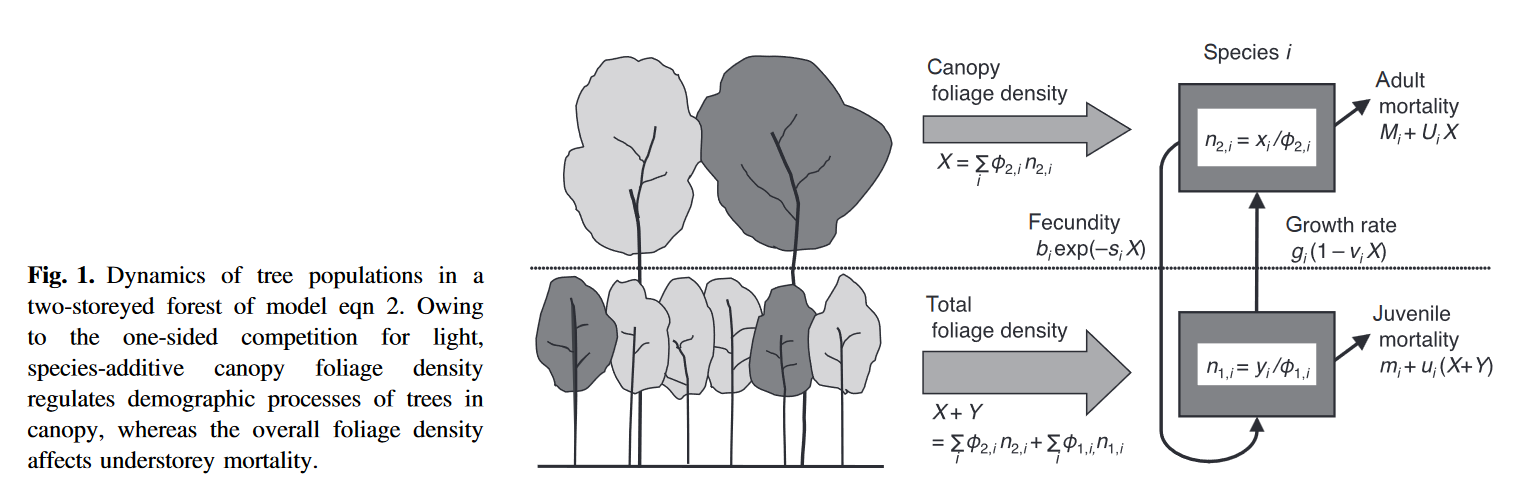
\includegraphics[width=\textwidth]{Figure/Fig_model_Kohyama.png}
    \caption{Figure from ~\autocite{kohyamaOnesidedCompetitionLight2012}}
    \label{fig:fig_model}
\end{figure}

Dynamic of each layer is driven by the competition from above layers foliage density (assimilated to the basal area) $\sum_{i = l}^{L} X_i$ with $X_i$ being the foliage density of layer $i$ :
\begin{equation}
    X_{l} = \sum_{sp} x_{sp,l} = \sum_{sp} \phi_{sp,l} n_{sp,l}
\end{equation}

The various processes are influenced by competition, with a linear negative relationship. Optimal probabilities are determined for each processes (birth $b$, growth $g$ and mortality $m$) without competition. These probabilities are then adjusted based on the process sensitivity ($Cb$, $Cg$, $Cm$) of the layer and species to foliage density.

\noindent The model can be summarised with one differential equation : \\
\begin{equation}\label{eq:model_general}
    \begin{split}
    \frac{dn_{sp,l}}{dt} = & 
    b_{sp,l} (1 - Cb_{sp,l} \sum_{i = 1}^{L} X_{i}) \\
    & + g_{sp,l - 1} \; n_{sp,l-1} (1 - Cg_{sp,l-1} \sum_{i = l-1}^{L} X_{i}) \\
    & - g_{sp,l} \; n_{sp,l} (1 - Cg_{sp,l} \sum_{i = l}^{L} X_{i}) \\
    & - m_{sp,l} \; n_{sp,l}(1 + Cm_{sp,l} \sum_{i = l}^{L} X_{i})
    \end{split}
\end{equation}
\\
And some special cases for lower and upper layers : \\
\begin{center}
    $b_{sp,l} = 0$ for l > 1 \\
    $g_{sp,L} = 0$ \\
    $g_{sp,0} = 0$
\end{center}

Population densities and demographic parameters are defined in ~\ref{tab:coef} and are all positive.

\begin{table}[H]
    \centering
    \begin{tabular}{l l l}
    \hline
    \hline
    \textbf{Abbreviation} & \textbf{Meaning} & \textbf{Unit} \\
    \hline
    \hline
    $l$            & layer index                                                 &          \\
    $L$            & number of layer (i.e. maximum layer)                        &          \\
    $sp$           & species index                                               &          \\
    $SP$           & number of species                                           &            \\
    $n_{sp,l}$     & number of trees of species $sp$ in layer $l$                & $ha^{-1}$  \\    
    $x_{sp,l}$     & foliage density of species $sp$ in layer $l$                & $m^2.ha^{-1}$  \\
    $\phi_{sp,l}$     & mean basal area of tree from species $sp$ in layer $l$    & $m^2$  \\
    $X_{l}$        & foliage density of layer $l$                                & $m^2.ha^{-1}$  \\ 
    $\sum_{i = l}^{L} X_{i}$     & foliage density above layer $l$      & $m^2.ha^{-1}$  \\ 
    $b_{sp}$       & optimal birth rate per tree in layer $L$    &  \\
    $Cb_{sp}$      & birth susceptibility to superior foliage density    & $ha.m^{-2}$           \\
    $g_{sp,l}$     & growth susceptibility to superior foliage density           &  \\
    $m_{sp,l}$     & probability of intrinsic mortality           & \\
    $Cg_{sp,l}$    & growth susceptibility to superior foliage density            &   $ha.m^{-2}$  \\
    $Cb_{sp,l}$    & mortality susceptibility to superior foliage density            & $ha.m^{-2}$    \\
    \hline
    \hline
    \end{tabular}
    \caption{Parameters for the model}
    \label{tab:coef}
\end{table}

\subsubsection{Model parametrisation}

We are starting with a 3 layers 3 species system with a mixture of possible species : \textit{Abies alba}, \textit{Betula pendula}, \textit{Fagus sylvatica}, \textit{Picea abies}, \textit{Pinus sylvestris}, \textit{Quercus pubescens}. The layers are defined by simplifying the IGN (French National Institute for Geographic and Forestry Information) 4-dimensional wood classification used in national forest inventory into 3 classes : dbh (cm) in [0,22.5] for small wood, [22.5,67.5] for medium and large, and [67.5+[ for very large. We have to define all parameters from the model.

Litterature and ForCEEPS simulations where used to adjust the dynamic of the system on a constant climate. (see appendix on parametrisation \autocite{bugmannEcologyMountainousForests1994,morinForestSuccessionGap2021}). Giving the parameters in Table S.\ref{tab:Final_param}.\\
We choose to concentrate our analyses on two species \textit{Abies alba} and \textit{Fagus sylvatica} as their dynamic was the most similar to ForCEEPS (REF to supplementary data) and they can be found together in mixed stand in France.\\

\subsection{Control theory and viability}

There doesn't seem to be any optimal solution to manage such complicated ecosystems, while taking into account their multi-functionality. Some methods, such as viability theory ~\autocite{aubinStochasticViabilityInvariance1990}, have been developed to actively discover sequences of actions sustaining multiple objectives within satisfaction constraints. Viability analyses establishes a framework to define control and states that can be combined to stay in our biological constraints for as long as needed \autocite{rougeExtendingViabilityTheory2013}.
Viability theory finds application in scenarios where objectives involve ecosystem services in forest social-ecological systems ~\autocite{mathiasUsingViabilityTheory2015, Houballah2021, Houballah2023}. In these studies, biodiversity is leveraged to identify viable control sequences, sustaining forest biodiversity and some ecosystem services through timber extraction control.
Nevertheless, it has not yet been employed to comprehend how controlling species diversity and selective disturbance targets can lead to viable management trajectories.

Viability theory provides a framework for management of dynamic systems. The challenge lies in finding management strategies (\(u(t)\)) that perpetually keep the system within a space of chosen constraints $K$. Rather than fixating on a single optimal state, the approach is to navigate within a spectrum of acceptable outcomes, preventing irreversible negative impacts.
In our case, the control is discrete and can happen every five years ($\Delta t$), mathematically, this is articulated as a controlled discrete-time dynamical system:

\[
N(t+\Delta t) = g(N(t), u(t), \Delta t),
\]

where \(N(t)\) is the system state at time \(t\), \(u(t)\) is the control applied at time \(t\), and \(g\) is the state transition function. In our case the state of the system, \(N(t)\), is defined by the matrix of the number of trees in each layer and for each species: \[ N(t) = [n_{sp,l}(t)]_{SP \times L} \]. And the state transition function is defined as the cut at discrete time t (\(u(t)\)) and the dynamic following it (described in Equation \eqref{eq:model_general}). The space of possible control is defined by the number of trees that are going to stay after a cut in the two higher layer :

\[
     U = \{u \in \mathbb{N}^{sp*Ncut} \mid \forall sp \in \mathbb{N}_{[1,SP]} \; \& \; l \in \mathbb{N}_{[c,L]}, u_{sp,l} \leq n_{sp,l}\}
\]

The space of possible control is then all the possible compositions of cut layers ($Ncut$ being the number of layers that are cut, 2 in our study, then the first layer cut is $c = L-Ncut+1 = 2$) such as the number of trees left is inferior to the number of trees present before the cut in the layer.\\

The resulting viability kernel (Viab(K)Viab(K)), which includes states where a management strategy can keep the system within desirable states, is formally described as:

\[
Viab(K) = \{N_0 \in K \mid\exists u(\cdot), \forall t \in \mathbb{N}_5, N(t) \in K\},
\]

where \(N_0\) denotes an initial state of the system in our constraints $K$. Within the viability kernel, at least one control strategy $u(\cdot)$ can maintain the system in a desirable state $K$. After the delimitation of the viability kernel all viable controls (\(u_v\)) can be determined and analysed.

To approach the viability kernel we used an algorithm inspired by Saint-Pierre (\autocite{saint-pierreApproximationViabilityKernel1994}).

To define the desirable states we chose constraints on wood extraction and diversity. The first one allow to take into account the economic aspect of forest management. The metrics for diversity were included as a way to take into account the diversity aspect of forest management and it's impact on other services. We chose to use the Shannon index as a measure of species and vertical diversity, as it is a common metric in ecology and combine information about diversity and evenness. \\
\\

After defining the viability kernel for : species...
Limits : we hae n points, values... nb of states + number of different control
Known limitation of the viability analyses (harware -> perhaps in discussion)
On a machin RAM, turning for blabla time with , code accessible at github; 
Everything ran with R 4 and analyses where also done with R. REF
We got the results :

\section{Results}

\subsection{Sensibility and Compatibility of the constraints}

\begin{figure}[h]
    \centering
    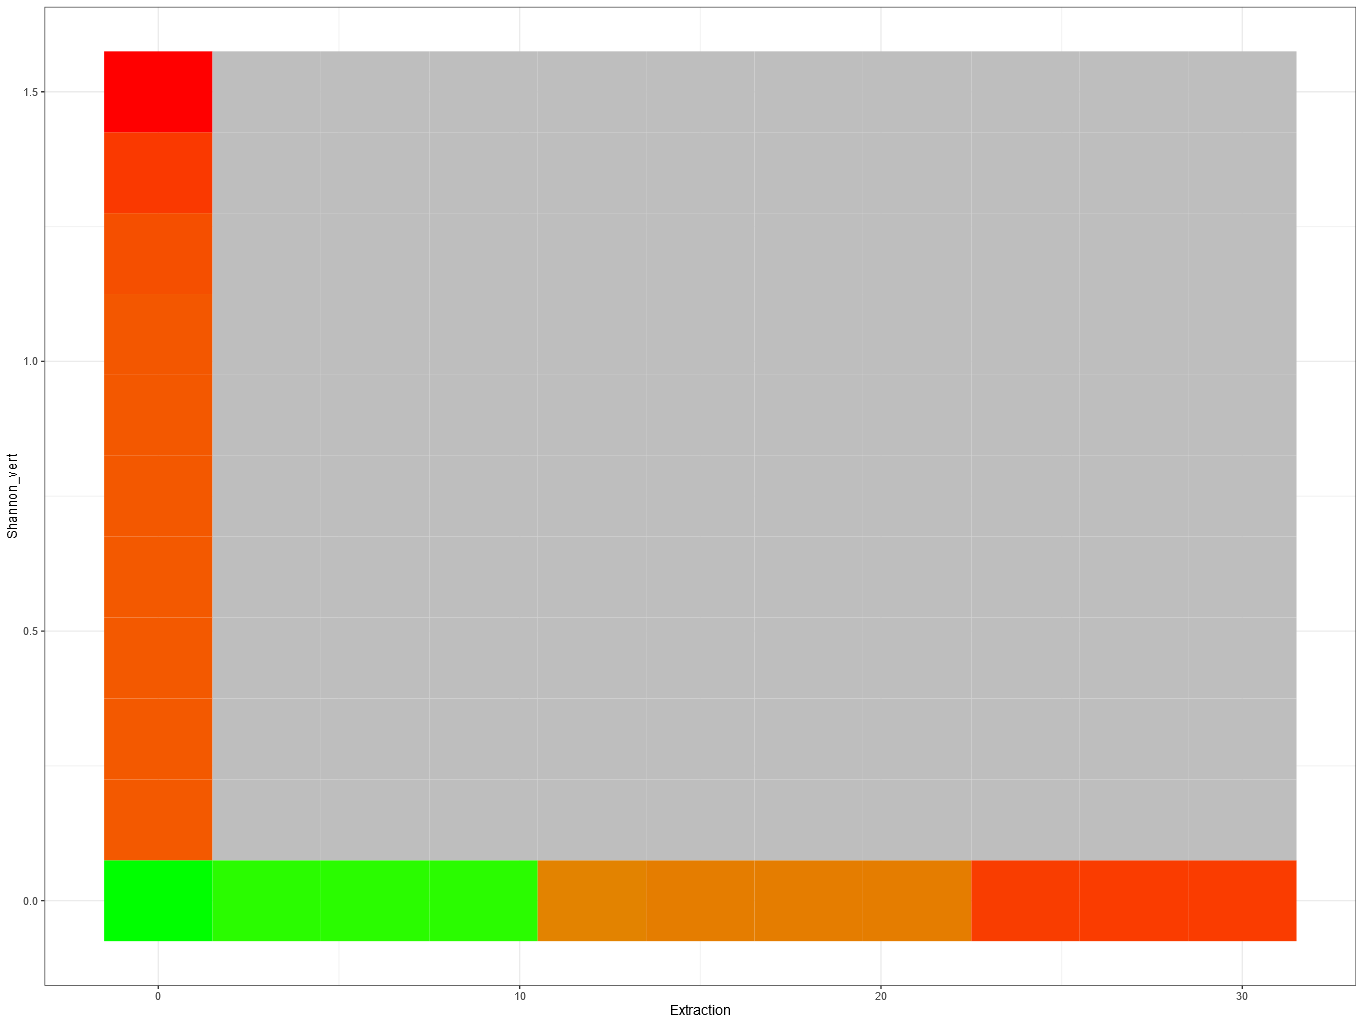
\includegraphics[width=\textwidth]{Figure/Sensi_ext_shvert.png}
    \caption{Figure : Volume of viability kernel function of constraints}
    \label{fig:sensi}
\end{figure}

\textbf{Conclusion} : If it is possible to stay inside a constraints of diversity both specific and vertical, as well as in a constraint of wood extraction, it is not possible to stay in a constraint of diversity and wood extraction at the same time.\\

Realistic constraints we chose to study : ... (But we already know that common constraints is not actually possible)

So we are going to compare the two

The question is then : what are the caracteristic of the two different viability kernel and what are the controls that can be applied to stay in one or the other ?.\\

\subsection{Viable state with diversity or wood extraction constraints : Volume and visualization, what in common ?}

\begin{figure}[h]
    \centering
    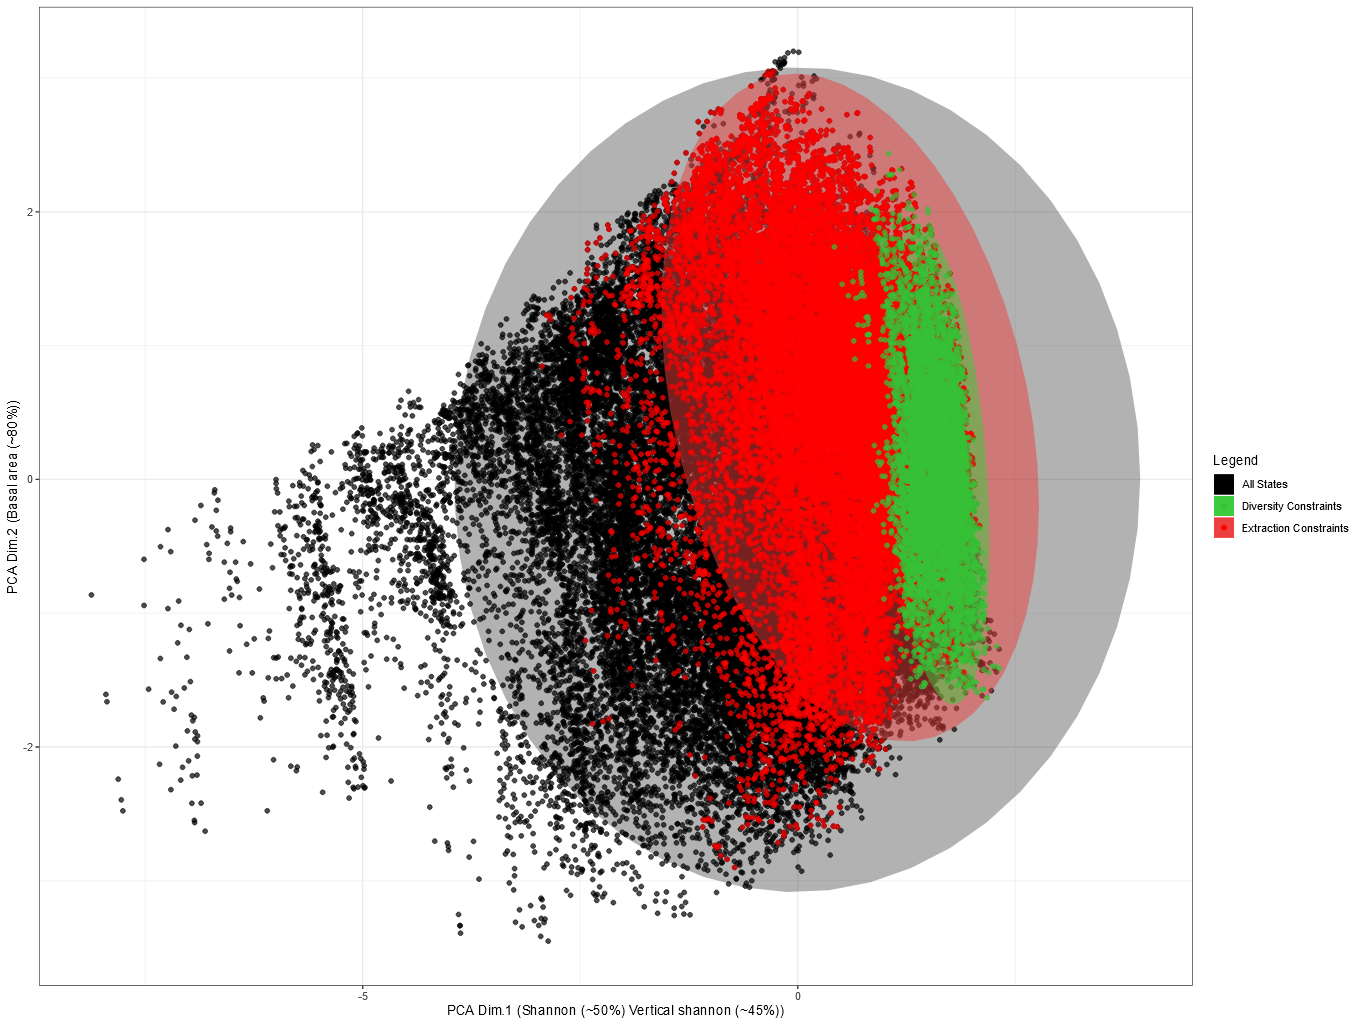
\includegraphics[width=\textwidth]{Figure/PCA_Viab_kernel_plot.png}
    \caption{Figure : Viable state in the PCA space (see appendix for PCA)}
    \label{fig:PCA_plot}
\end{figure}

Volume of viability kernel : \\

\begin{table}[H]
    \centering
    \begin{tabular}{l l l l l}
    \hline
    \hline
    \textbf{Constraints} & \textbf{State} & \textbf{Post control state} & \textbf{Control state} & \textbf{Association} \\
    \hline
    Diversity  & 6 285 & 1 455 & 320 & 106 735 \\
    Extraction & 11 899 & 8 756 & 622 & 349 037 \\
    Shared & 6 121 & 1 193 & 1 317 & 61 144 \\  
    Total     & 15 625 & 15 625 & 625 & 1.3 Million \\
    \hline
    \hline
    \end{tabular}
    \caption{Volume of the viable space}
    \label{tab:Viab_volume}
\end{table}

\textbf{Conclusion} : A lot of common state even though there is an incompatibility between the two constraints.Perhaps on a limited timeline it is possible to stay in both constraints.\\

\subsection{Viable state with diversity or wood extraction constraints : caracteristic comparaison}

\begin{figure}[h]
    \centering
    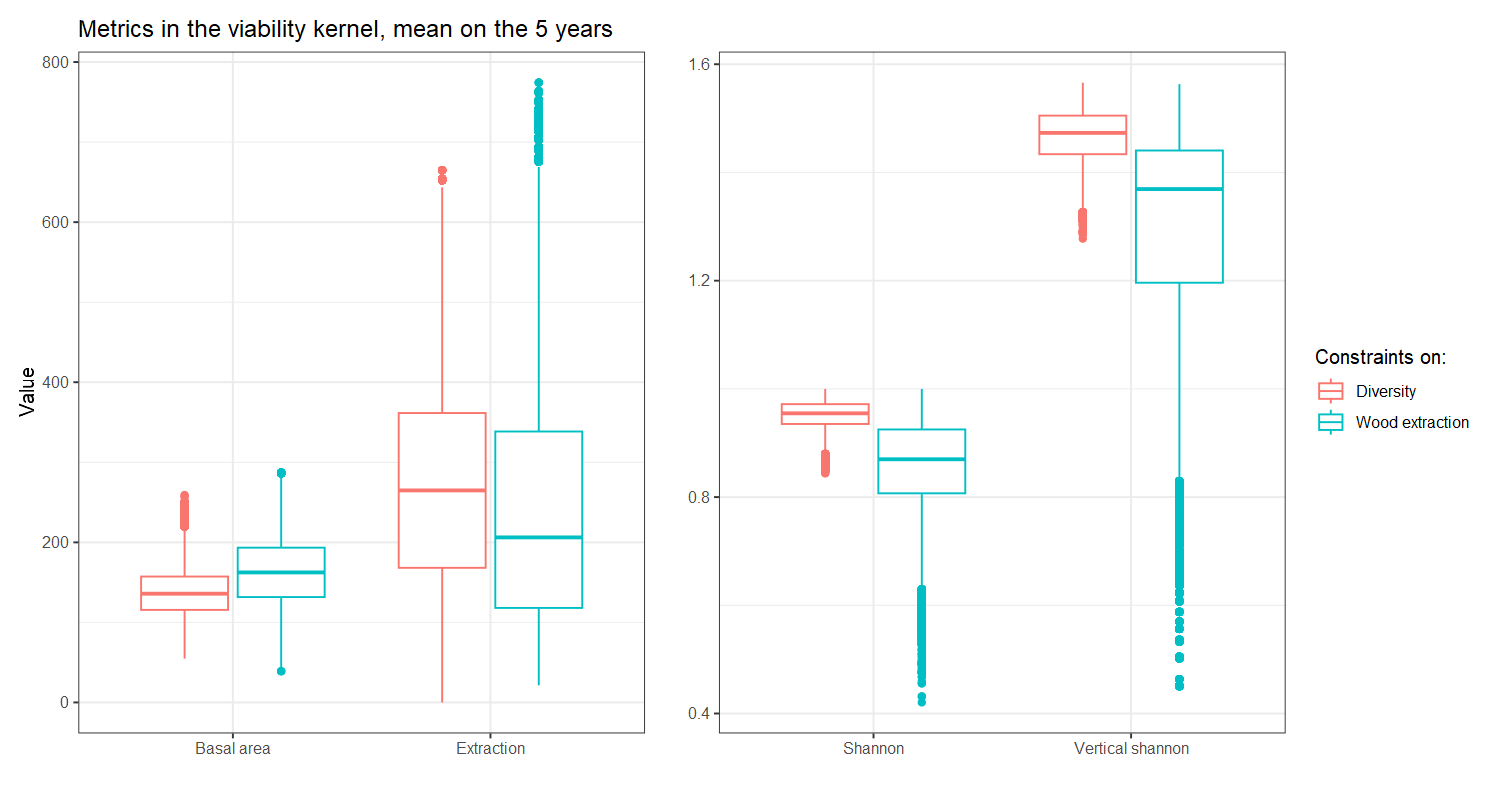
\includegraphics[width=\textwidth]{Figure/Viab_metric_mean.png}
    \caption{Figure : Metric in the viable state}
    \label{fig:Viab_metric_comp}
\end{figure}

\textbf{Conclusion} : Questions on volume, is it possible to cut so much (necessity of an upper limit + verif of formula for wood volume). Seems that there is no huge sacrifice of wood extraction for diversity, but mean doesn't take into account potential attraction inside the viability kernel.\\

\subsection{Viable control with diversity or wood extraction constraints}

Control as in state and what we extract ?
Different betwwen both, nb of viable control : diversity () and extraction ()

Caracteristic of common state and/or control ?\\

\section{Discussion for now random text on reflexion I had and may be incliduded or not}

The limit of this kind of studies is their computational cost, and the need for a simple model, which means a compromise between complexity and realism. Our first hypothesis is that we can use a theoretical model to explore the effect of diversity on ecosystem services, and that the results will be transferable to more complex models.

Landscape diversity

Limit of parametrisation : other possibilities : data/ easy abc, error, sensitivity analysis, and also more generally simplified model truthtfullness

Limit : choice of diversity index, sensibility and Hill number, Gini...

\subsection{Forest diversity, may be more complex than diversity drives diversity}

In forests diversity can be define in different ways : Composition or structural diversity. And at different scale from the stand to the landscape.\\
Work on composition diversification and its effects is mainly driven by the first work on biodiversity ecosystem functioning (BEF) from grassland studies ~\autocite{tilmanBiodiversityPopulationEcosystem1996}.They showed that there was a positive link between biodiversity and ecosystem functioning. But the mechanisms behind this link are still not well understood. Numerous hypothesis were made to explain this link: competitive exclusion, niche complementary, sampling effect, etc. ~\autocite{aliBiodiversityEcosystemFunctioning2023}. This uncertainty makes it difficult to predict the impact of biodiversity loss, and even more in other ecosystems than grasslands.
While the hypothesis of BEF relationship, and its relevance is still debated, it fuels an entire segment of research.
The study of BEF in forest is more recent and mainly focused on the link between species diversity and productivity. A positive relationship has been demonstrated at a global scale ~\autocite{liangPositiveBiodiversityproductivityRelationship2016}, but also in specific forest ~\autocite{morinTreeSpeciesRichness2011,paquetteEffectBiodiversityTree2011,jourdanManagingMixedStands2021}. But as for grassland the mechanisms are not understood and the interaction is not positive in every forest type. ~\autocite{forresterReviewProcessesDiversity2016}.
However one of the way to explain the contrasting results could be that the biodiversity-productivity interaction is context dependant. The relationship seems to be mostly positive in harsh climate and low tree density but negative in suitable environment ~\autocite{juckerClimateModulatesEffects2016}.

It is also reductive to consider productivity as the only characteristic of forest ecosystems, and many other should be accounted for : support of habitat and biodiversity, regulation of flood, carbon storage and also cultural and aesthetic values.
All of them might not be impacted in the same way ~\autocite{korboulewskyHowTreeDiversity2016}.
To have a better understanding of the impact of biodiversity on forest functioning it seems necessary to study multiple functions at the same time. It has been shown that diversity can increase multi-functionality by the jack-of-all-trades mechanism ~\autocite{vanderplasJackofalltradesEffectsDrive2016} while not optimizing any of them. This compromise can be seen in the balance between young and old grown forests, if the firsts are more productive, they store less carbon than the last ~\autocite{caspersenSuccessionalDiversityForest2001}. It is thus important to define the functions that we want to preserve as well as threshold for each of them.

Actually species diversity is not the only way to bring back diversity in forest and recently vertical diversity in forest have also been advocated to be a possible solution to the increasing vulnerability of this ecosystem ~\autocite{guldinRoleUnevenAgedSilviculture1996}. Today only 25\% of managed forest in Europe is composed of uneven aged stand (foresteurope.org), but the actual effect of such management is hardly consensual. In his review in 2017 Nolet ~\autocite{noletComparingEffectsEven2018} concludes that "overall, the complexity	of comparing even- and uneven- aged silviculture may explain the surprisingly limited number of studies that compare ecological effects of even- and uneven- aged silviculture".

\subsection{Plantation}

Forest management encompasses more than just harvesting; it involves considerations such as plantation practices, which can directly address questions related to species choice and turnover in the face of climate change. The intricate dynamics of species selection become a crucial consideration, presenting a potential advantage in the context of forest plantation management (\autocite{brockerhoffPlantationForestsBiodiversity2008}). Furthermore, the exploration extends to the conversion to uneven shelterwood practices, prompting research inquiries into the optimal methodologies involved (\autocite{sinhaOptimalManagementNaturally2017,dudumanForestManagementPlanning2011,nylandEvenUnevenagedChallenges2003}).

\clearpage

\printbibliography

\clearpage

% title page : Appendix

\begin{center}
    \textbf{\Large Appendix}
\end{center}

\pagenumbering{roman}
\appendix

\section{Kohyama model parametrisation}

We are starting with a 3 layers 3 species system with a mixture of possible species : \textit{Abies alba}, \textit{Betula pendula}, \textit{Fagus sylvatica}, \textit{Picea abies}, \textit{Pinus sylvestris}, \textit{Quercus pubescens}. The layers are defined by dbh (cm) interval : [0,22.5], [22.5,67.5], [67.5+[. We have to define all parameters in Table \ref{tab:coeftoparam}.

\begin{table}[H]
    \centering
    \begin{tabular}{l l l}
    \hline
    \hline
    \multicolumn{3}{l}{\textbf{By species}, $sp$} \\
    \hline
    $b_{sp,1}$     & optimal birth probability                              & $ha^{-1}.year^{-1}$ \\
    $Cb_{sp,1}$    & birth susceptibility to superior foliage density       & $ha.m^{-2}$       \\
    $m_{sp}$       & probability of intrinsic mortality                     & $year^{-1}$ \\
    $Cg_{sp}$      & growth susceptibility to superior foliage density      & $ha.m^{-2}$           \\
    $Cm_{sp}$      & mortality susceptibility to superior foliage density   & $ha.m^{-2}$           \\    
    \\
    \multicolumn{3}{l}{\textbf{By layer $l$}} \\
    \hline
    $\phi_{l}$  & mean basal area per tree in layer $l$        & $m^{2}.ha^{-1}$  \\
    \\
    \multicolumn{3}{l}{\textbf{By species $sp$ and layer $l$}} \\
    \hline
    $g_{sp,l}$     & optimal probability of transition from layer $l$ to the next & $.year^{-1}$ \\
    \\
    \hline
    \hline
    \end{tabular}
    \caption{Parameters that we have to define numerically}
    \label{tab:coeftoparam} 
\end{table}

\subsection{Parameters deduced form litterature of ForCEEPS and ForClim}

\subsubsection{Basal area}

Basal area is defined as the area of the cross subsection of the tree at breast height (1.3m). It is a good indicator of the density of the forest. It is defined as : 

\begin{equation}
    \phi_{l} = \frac{\pi}{4} * \overline{D_{l}}^2
\end{equation}

With $\overline{D_{l}}$ the mean diameter in layer $l$. (i.e. 11.25, 45, 100 cm).\\

\subsubsection{Intrinsec Mortality}

Mortality was defined axactly as in ForCEEPS, as the inverse of the life expectancy of the species ($A_{max}$) multiplied by a factor $c_{mort}$ = 4.605.
\begin{equation}
    m_s = \frac{c_{mort}}{A_{max_s}}
\end{equation}

$A_max$ can be found in the thesis on ForClim \autocite{bugmannEcologyMountainousForests1965} or the supplementary data of ForCEEPS \autocite{morinForestSuccessionGap2021}

\subsubsection{Optimal Growth}

Optimal growth is defined in ForCEEPS \autocite{morinForestSuccessionGap2021} as :

\begin{equation}
    \Delta D_{\mathrm{opt}_i}(t+1)=g_s \frac{D_i(t)\left(1-\frac{H_i(t)}{H_{\max _s}}\right)}{2 H_{\max _s}-b_{\max _s} \times \exp \left(\left(\frac{-s_s}{b_{\max _s}} D_i(t)\right) \times\left(\frac{-s_s}{b_{\max _s}} D_i(t)+2\right)\right.}
\end{equation}

With $g_s$ the growth rate, $D_i$ the diameter of the tree, $H_i$ the height of the tree, $H_{\max _s}$ the maximum height of the species, $b_{\max _s}$ the maximum heigth of the species above breast ($b_{\max _s} =  H_{\max _s} - 1.37$), and $s_s$ the shape parameter of the species. $g_s$, $H_{\max _s}$, and $s_s$ can be found in the appendix \autocite{morinForestSuccessionGap2021}. $H_i$ is also defined as a function of $D_i$ :

\begin{equation}
    H_i(t)=b+b_{\max _s}\left(1-\exp \left(-\frac{s_s}{b_{\max _s}} D_i(t)\right)\right)
    \label{eq:height}
\end{equation}

This gives a function $f(D_i) = \Delta D_{\mathrm{opt}_i}(t+1)$, which is the growth of the tree as a function of its diameter.

\begin{figure}
    \centering
    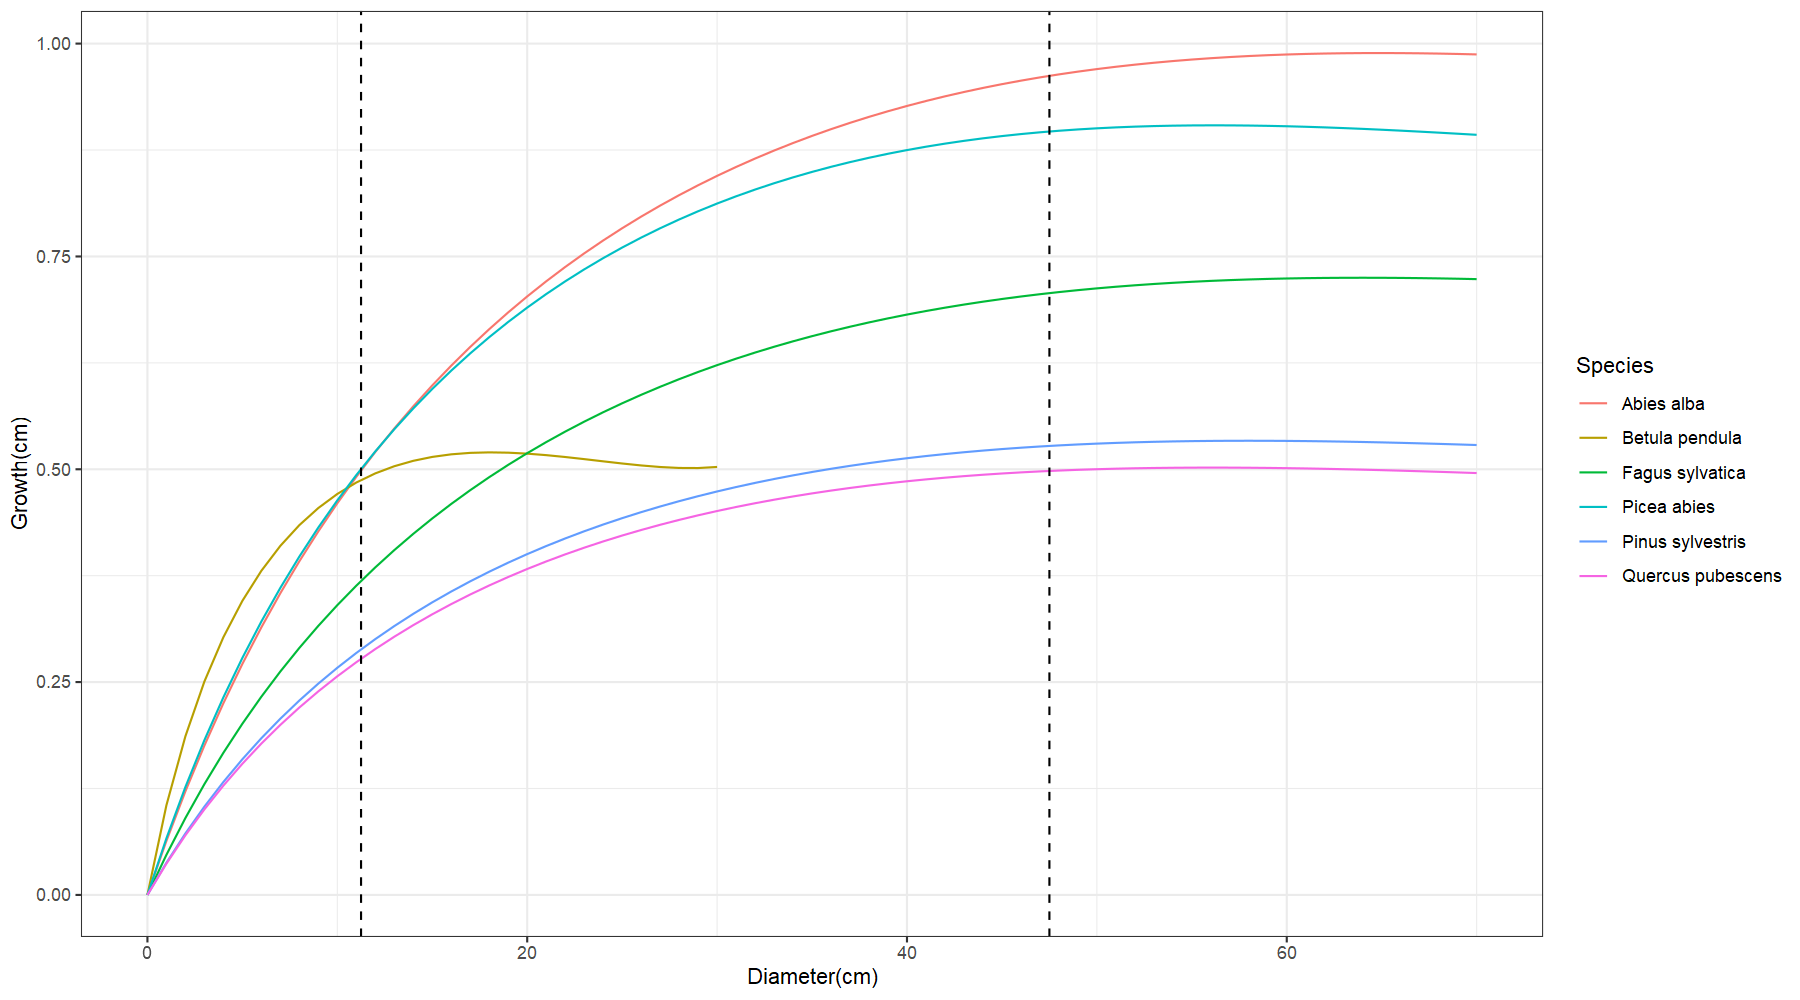
\includegraphics[width=\textwidth]{Figure/Growth_diameter.png}
    \caption{Growth as a function of diameter for the 5 species}
    \label{fig:growth_diameter}
\end{figure}

As our model does not account for a change of growth with diameter we took the growth from the mean diameter of our two interval : [0, 22.5] and [22.5, 67.5] (i.e. 11.25 and 45). It gives :

\begin{table}[H]
\begin{center}
    \begin{tabular}{lll}
    \hline
    Species & Growth 1 & Growth 2 \\ \hline
    \textit{Abies alba} & 0.5 & 0.96 \\
    \textit{Betula pendula} & 0.5 & 0 \\
    \textit{Fagus sylvatica} & 0.37 & 0.71 \\
    \textit{Picea abies} & 0.5 & 0.9 \\
    \textit{Pinus sylvestris} & 0.29 & 0.53 \\
    \textit{Quercus pubescens} & 0.28 & 0.5 \\ \hline
    \end{tabular}
    \caption{Growth for the 5 species and two below layers}
\end{center}
\end{table}

Growth is the number of cm added to the diameter of the tree each year. To get the transition probability to the next layer with the assumption that tree dbh are uniformly distributed in each layer we need to divide this value by the diameter difference of the layer (See Tab. \ref{tab:final_param}).

\subsubsection{Optimal Esthablishment}

Establishment is a process that is still not well understood. In ForCEEPS optimal establishment (if all the threshold for establishment are met) is the same for every species : 0.006 individu/m2/year. We will use this value for our model for every species.

\subsubsection {Light competition}

Proportionality between the species is known (see ForClim Ly (growth) and La(birth)), as mortality due to light competition is due to the absence of growth we used the same proportionality between species.

\begin{table}[H]
\begin{center}
    \begin{tabular}{lll}
    \hline
    Species & Ly (growth, mortality) & La (birth) \\ \hline
    \textit{Abies alba} & 0.05 & 1 \\
    \textit{Betula pendula} & 0.3 & 9 \\
    \textit{Fagus sylvatica} & 0.05 & 1 \\
    \textit{Picea abies} & 0.1 & 5 \\
    \textit{Pinus sylvestris} & 0.3 & 9 \\
    \textit{Quercus pubescens} & 0.3 & 7 \\ \hline
    \end{tabular}
    \caption{Sensitivity for light competition}
    \label{tab:prop_sensitivity}
\end{center}
\end{table}

If we have a relative sensitivy of our species to light availability we still have to get the global coefficient linked to this sensitivity for growth, birth and mortality. We cannot extract the parameters from a simplification as we used a negative linear function, which is not the case in ForCEEPS. We will use the data from ForCEEPS to fit our parameters.

\subsection{ForCEEPS input data and results}

ForCEEPS simulations where used to adjust the dynamic of the system. 6 species where chosen to do so : \textit{Abies alba}, \textit{Betula pendula}, \textit{Fagus sylvatica}, \textit{Picea abies}, \textit{Pinus sylvestris}. We chose a constant climate for 300 years drawn randomly from meteorologic data from Bern between 1950 and 2000 (resulting climate can be found in Fig. \ref{fig:climate}). We used the same initial forest structure for all simulations : 10 trees per species per layer. We did 20 simulations of 1000m2 patch for each species association. We then took the mean of the 20 simulations and multiplied it by 10 to get the number of trees per hectare. We then fitted the parameters of the model to get the same dynamic as the ForCEEPS simulations.

\subsubsection{Climate}

Climate was taken randomly for each months in the climate data from 1950 to 2000 (Bern), to get a constant climate. To be sure to have non limiting precipitation they were all multiplied bya factor 10.

\begin{figure}[H]
    \centering
    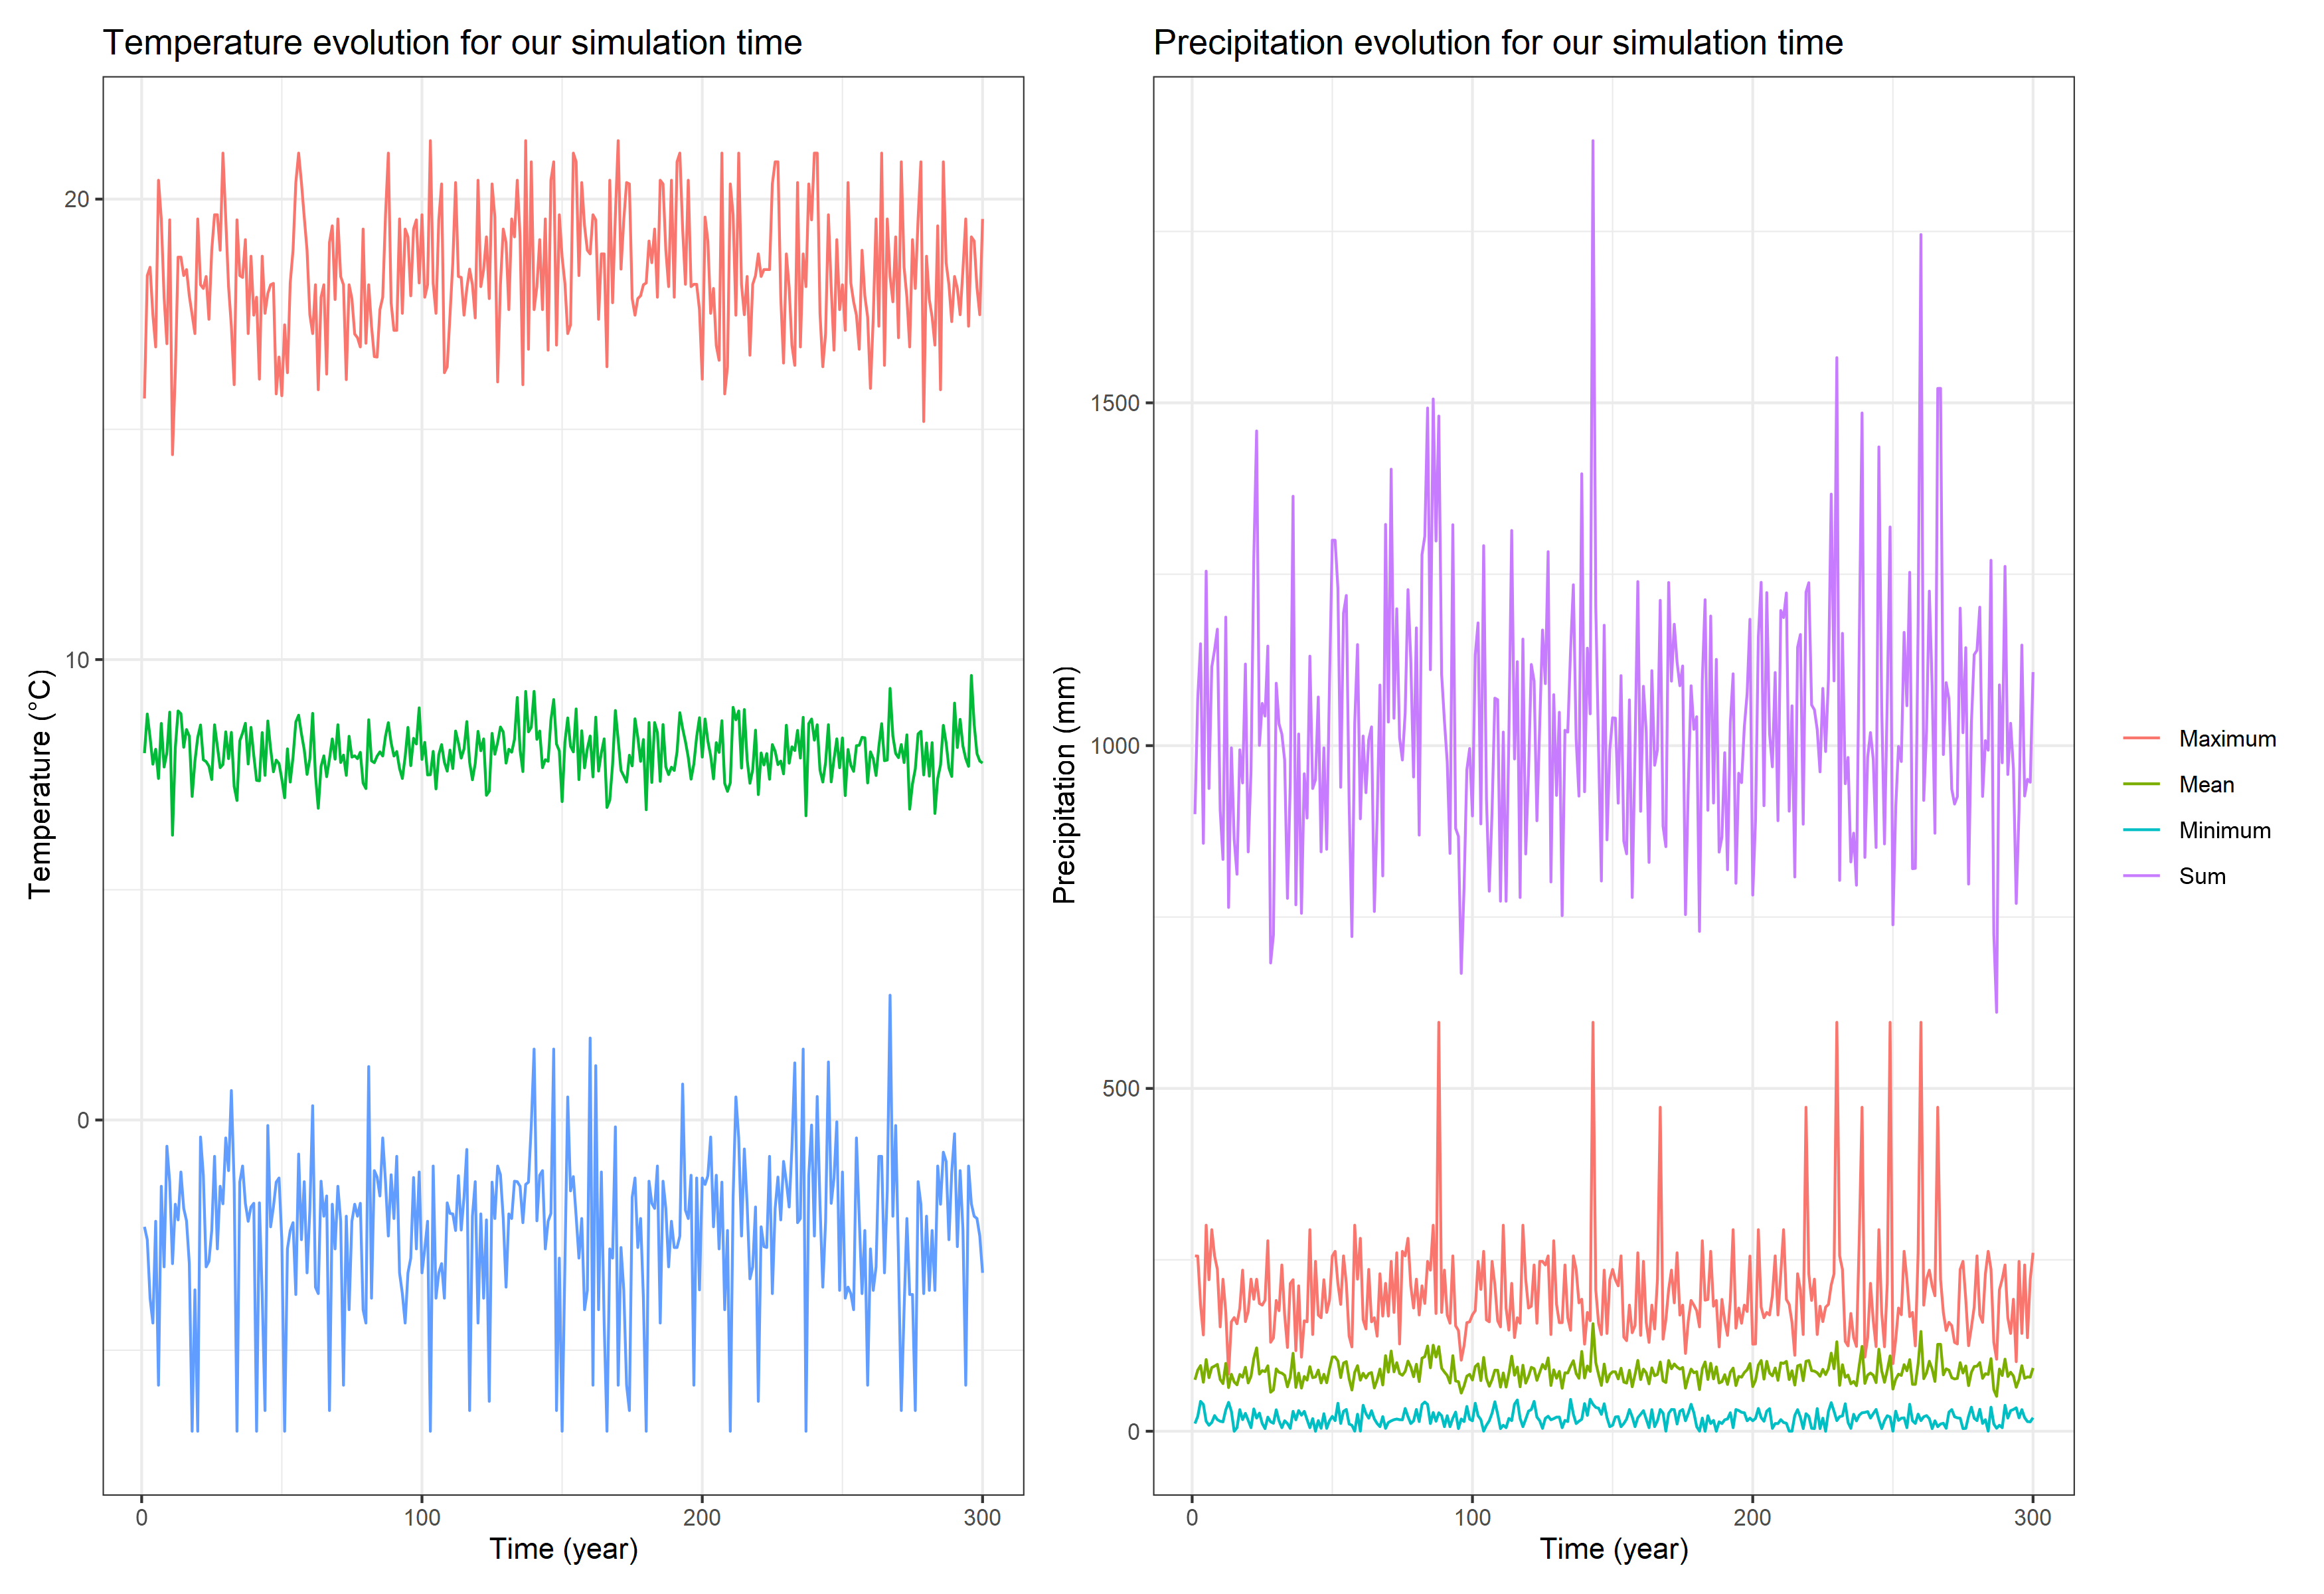
\includegraphics[width=1\textwidth]{Figure/Climate_simul.png}
    \caption{Climate for our ForCEEPS simulation}
    \label{fig:climate}
\end{figure}

\subsubsection{setup parameters}

For the setup parameters we used non limiting values for water and nitrogen. The parameters can be found in the github documents (file Basic.setup), and are the same for all simulations.

Result of the simulation are in color in Fig. \ref{fig:Simulation_fit}.

\subsubsection{Fitting the parameters}

To fit the parameter we used the function optim in R with the following parameters :

\begin{tcolorbox}
result <- optimParallel(start point, function to minimize, lower = rep(0,3), upper = rep(0.1,3), method = ''L-BFGS-B'')
\end{tcolorbox}

Method "L-BFGS-B" (see optim documentation ~\url{https://www.rdocumentation.org/packages/stats/versions/3.6.2/topics/optim}) allows box constraints, that is each variable can be given a lower and/or upper bound. The initial value must satisfy the constraints. This uses a limited-memory modification of the BFGS quasi-Newton method.  "BFGS" is a quasi-Newton method (also known as a variable metric algorithm), specifically that published simultaneously in 1970 by Broyden, Fletcher, Goldfarb and Shanno. This uses function values and gradients to build up a picture of the surface to be optimized.

I only fit three non specific parameters LCg (light competition for growth), LCm (light competition for mortality) and LCb (light competition for birth). In the model they are then multiplied by the sensitivity of the species to light competition (see Tab. \ref{tab:prop_sensitivity}).

\subsubsection{Results}

% figure sur toute une page dans le sens de la longueur (landscape)
\begin{sidewaysfigure}[ht]
    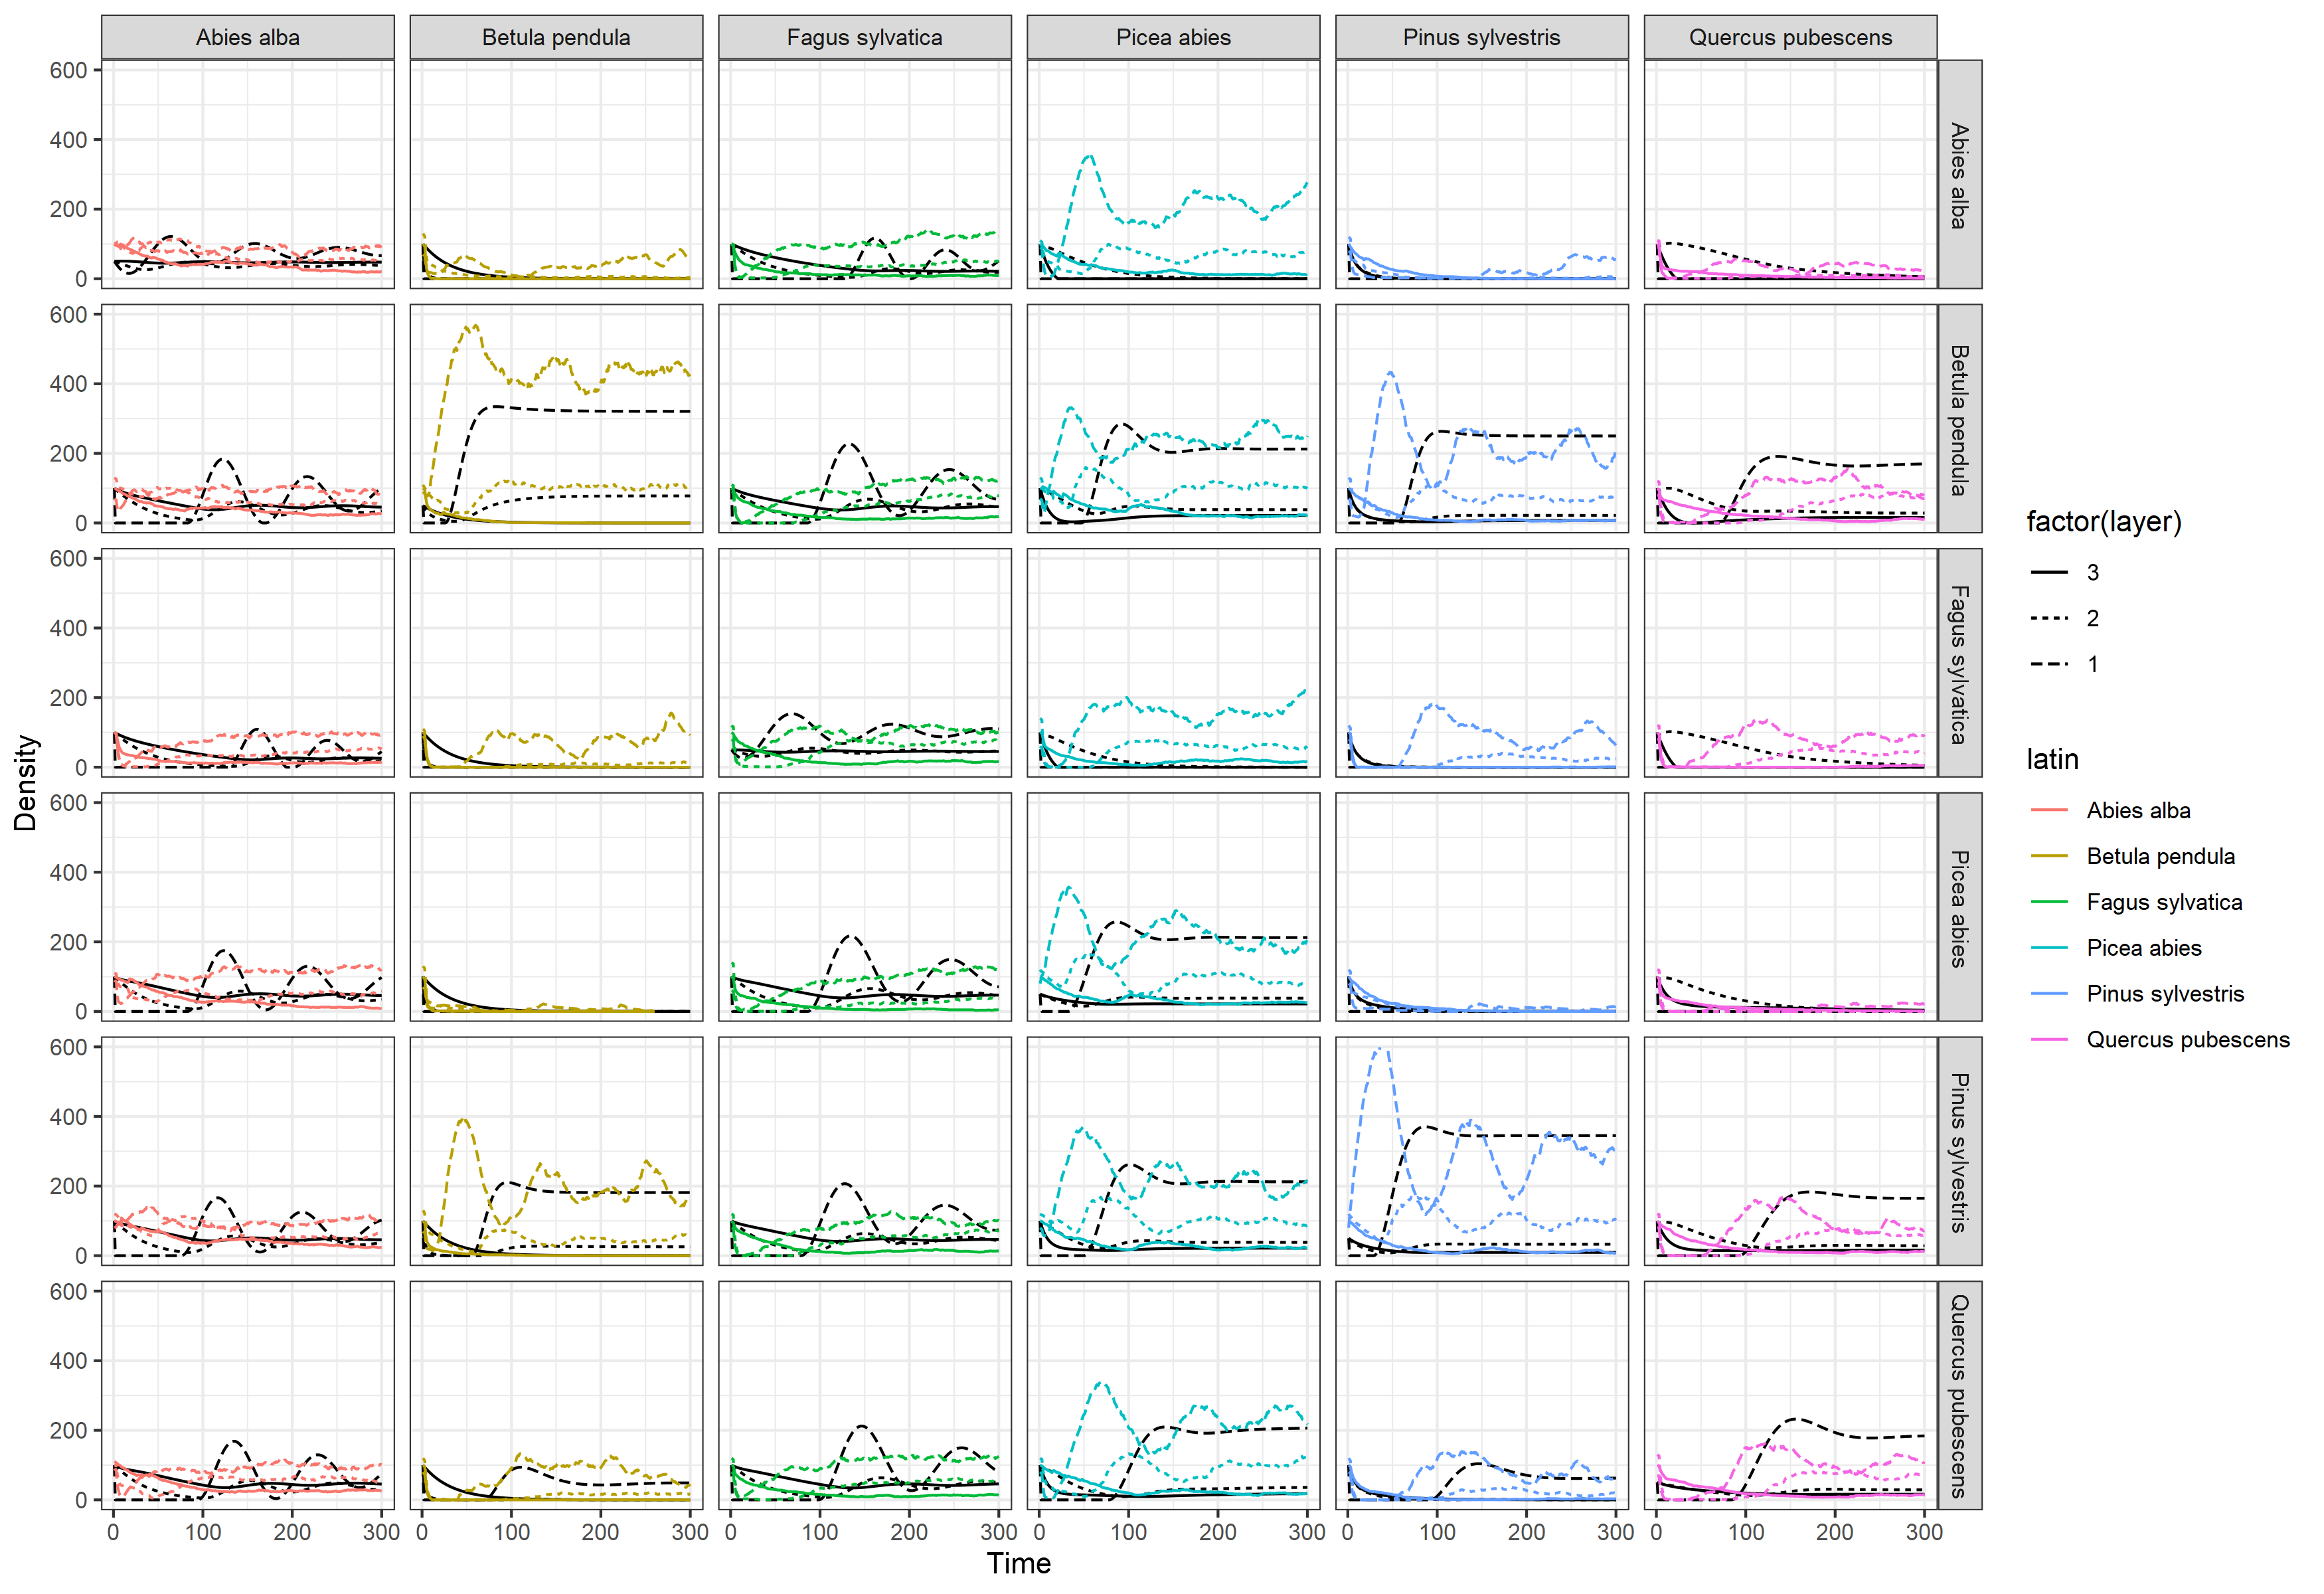
\includegraphics[width=\textwidth]{Figure/Simulation_fit.png}
    \caption{Fit Kohyama model (color) on ForCEEPS simulation (black) for individual species}
    \label{fig:Simulation_fit}
\end{sidewaysfigure}

\begin{table}[H]
\begin{center}
    \begin{tabular}{llllllll}
    \hline
    Species & b (/ha/an) & m (/year) & g1 (/year) & g2 (/year) & LCb & LCm & LCg \\ \hline
    \textit{Abies alba}       & 60 & 0.013 & 0.022 & 0.021 & 0.0059 & 0.0046 & 0.0059 \\
    \textit{Betula pendula}   & 60 & 0.031 & 0.022 & 0     & 0.0295 & 0.0229 & 0.0295 \\
    \textit{Fagus sylvatica}  & 60 & 0.012 & 0.016 & 0.016 & 0.0531 & 0.0413 & 0.0531 \\
    \textit{Picea abies}      & 60 & 0.015 & 0.022 & 0.02  & 0.0531 & 0.0413 & 0.0531 \\
    \textit{Pinus sylvestris} & 60 & 0.023 & 0.013 & 0.012 & 0.0059 & 0.0046 & 0.0059 \\
    \textit{Quercus pubescens}& 60 & 0.008 & 0.012 & 0.011 & 0.0413 & 0.0321 & 0.0413 \\ \hline
    \end{tabular}
    \caption{Parameters found for the 5 species}
    \label{tab:Final_param}
\end{center}
\end{table}

\subsection{Volume allometry}

Volume was calculated with the formula from \autocite{deleuzeEstimerVolumeTotal2014} :

\begin{equation}
    \text { VolTot }=\frac{h_{\text {tot }} \cdot c_{130}{ }^2}{4 \pi\left(1-\frac{1.3}{h_{\text {tot }}}\right)^2}\left(a+b \cdot \frac{\sqrt{c_{130}}}{h_{\text {tot }}}+c \cdot \frac{h_{\text {tot }}}{c_{130}}\right)
\end{equation}

With $h_{tot}$ the total height of the tree, $c_{130}$ the diameter at 130cm, and $a$, $b$, and $c$ the coefficients for each species. The coefficients can be found in \autocite{deleuzeEstimerVolumeTotal2014}. $h_tot$ was defined as a function of $c_{130}$ like in equation \ref{eq:height}. 

\begin{table}[h]
    \centering
    \begin{tabular}{lccc}
    \hline
    \hline
    \textbf{Species} & \textbf{Volume layer 1} & \textbf{Volume layer 2} & \textbf{Volume layer 3} \\
    \hline
    \textit{Abies alba} & 0.007624415 & 0.2518305 & 1.724068 \\
    \textit{Picea abies} & 0.009195898 & 0.2779880 & 1.697751 \\
    \textit{Pinus sylvestris} & 0.005440307 & 0.1669922 & 1.134001 \\
    \textit{Betula pendula} & 0.004805793 & 0.1585726 & 0.947111 \\
    \textit{Fagus sylvatica} & 0.005384323 & 0.2140528 & 1.681878 \\
    \textit{Quercus pubescens} & 0.004872535 & 0.1729537 & 1.281115 \\
    \hline
    \hline
    \end{tabular}
    \caption{Volume of the 6 species in the 3 layers (m3/tree)}
    \label{tab:volume}
\end{table}

\end{document}